\documentclass[11pt,letterpaper]{article}
\usepackage[utf8]{inputenc}
\usepackage[spanish]{babel}
\usepackage{amsmath}
\usepackage{amsfonts}
\usepackage{amssymb}
\usepackage{graphicx}
\usepackage{lmodern}
\usepackage{tikz,pgf}
\usepackage{mathrsfs}
\usetikzlibrary{arrows}
\title{Pequeño aporte}
\author{Germán Avendaño Ramírez}
\begin{document}
\maketitle
En el caso del primer ejercicio
\[f(x)=\left\{ \begin{array}{lcl}
\dfrac{ax^{2}-2}{x-4} & \mbox{si} & x> 3\\
-x & \mbox{si} & x< 3\\
\end{array}
\right. \]
Esta función será continua en un intervalo que contenga a 3, si los límites laterales son iguales (\textit{por izquierda y derecha}),  es decir si:
\[\displaystyle{\lim_{x\rightarrow 3^{-}}f(x)=\lim_{x\rightarrow 3^{+}}f(x)}\]
Es decir si:
\begin{align*}
\displaystyle{\lim_{x\rightarrow 3}-x}&=\displaystyle{\lim_{x\rightarrow 3}\dfrac{ax^{2}-2}{x-4}}\\
-3&=\dfrac{a(3^{2})-2}{3-4}\\
-3(-1)&=9a-2\\
3+2&=9a\\
a&=\frac{5}{9}
\end{align*}
Por tanto para que la función $f$ sea continua en la vecindad de $x=3$, $a$ debe ser igual a  $\frac{5}{9}$, tal como se puede ver en la gráfica de geogebra.

\begin{center}
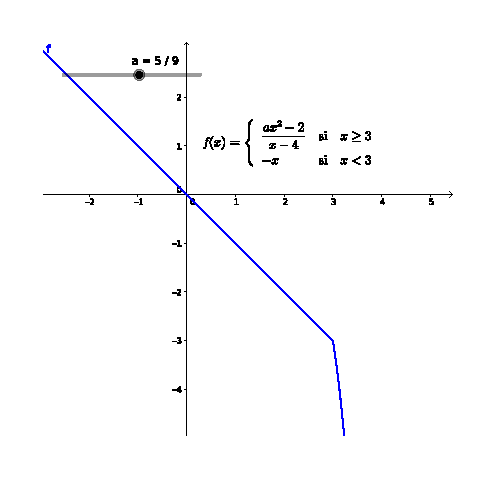
\includegraphics[scale=1.25]{Images/angela} 
\end{center}
De manera similar puede uno hacer con los demás ejercicios, para estar seguro al resolverlo también algebraicamente.

En el caso del segundo ejercicio, le adjunto un archivo de geogebra \textit{angela.ggb}. A esta función la he denominado $g$ para diferenciarla del primer ejercicio. En este caso el valor de $a$ debe estar alrededor de 28.2 o 28.25, habría que comprobarse algebraicamente.

Me place tener noticias suyas Angelita. Un beso y un abrazo.
\end{document}